\documentclass[acmtog, screen]{acmart}

\usepackage[utf8]{inputenc}
\usepackage[spanish]{babel}
\usepackage{graphicx}
\graphicspath{{../fig/}}

\usepackage{booktabs} % For formal tables
\usepackage{hyperref}

% Document starts
\begin{document}
% Title portion
\title{Desarrollo de Sistemas Inteligentes - Trabajo de clustering}

\author{Luis Cabañero Gómez}
\email{Luis.Cabanero@alu.uclm.es}

\maketitle

Enlace a repositorio GitHub: \url{https://github.com/Xiul109/DSI}

Enlace a vídeo de Youtube: \url{https://youtu.be/rrquQzMpz5M}

\section{Introducción}
Este documento describe el proceso que se ha seguido par analizar datos de las rentas por municipios\footnote{\url{http://www.fedea.net/renta/}} del año 2007 mediante técnicas de clustering, así como los resultados que se han obtenido. El proceso se ha dividido en dos etapas: preprocesado y clustering. Como herramienta para realizar el clustering se utilizarán mapas autoorganizados de Kohonen.

\section{Preprocesado}
En esta etapa se han analizado los datos en profundidad para determinar cuáles son los campos más relevantes para este problema, así como hacer una limpieza de los mismos. Para esta primera fase se ha utilizado Python como lenguaje de programación, principalmente por tener mayor conocimiento del mismo. Se han utilizado los módulos: pandas, numpy, matplotlib, seaborn y scikit-learn. El preprocesado se puede ejecutar mediante el script ``preprocesado.py''.

El primer paso ha sido cargar el fichero, cosa que no ha sido inmediata debido a que las primeras filas no correspondían a las cabeceras de los campos. De primeras se han eliminado los campos ``Código INE municipio (5 dígitos)'' , ``Código INE Provincia '' y ``Código INE Comunidad Autónoma '' debido a que la información que contienen no es muy relevante y en el caso de los códigos de municipio y provincia son, además, redundantes. Además de eliminar esas columnas se han eliminado unas 8 filas a las que les faltaba información en algunos campos y se han convertido los campos numéricos a tipo float, ya que por defecto se interpretaron como texto.

El siguiente paso ha sido añadir coordenadas geográficas a los datos, los cuales se utilizarán más adelante para mostrar la localización de diversos municipios. Esto se ha hecho relacionando el código INE del municipio de los datos de la renta con otra tabla que incluye información sobre la situación geográfica\footnote{\url{http://centrodedescargas.cnig.es/CentroDescargas/equipamiento.do?method=descargarEquipamiento\&codEquip=8}}. Una vez añadidos las columnas con la información de la longitud y la latitud, se ha eliminado el campo ``Código INE municipio'', ya que no será necesario más adelante.

\subsection{Selección de campos}
El siguiente paso ha sido estudiar las correlaciones entre los diferentes campos numéricos. En la figura \ref{fig:correlaciones1} pueden verse estas correlaciones de manera gráfica. Con ayuda de estas correlaciones y mediante la semántica de los datos se ha podido determinar qué campos pueden quitarse de cara al clustering final. Las conclusiones que se han sacado han sido los siguientes:

\begin{figure}
	\centering
	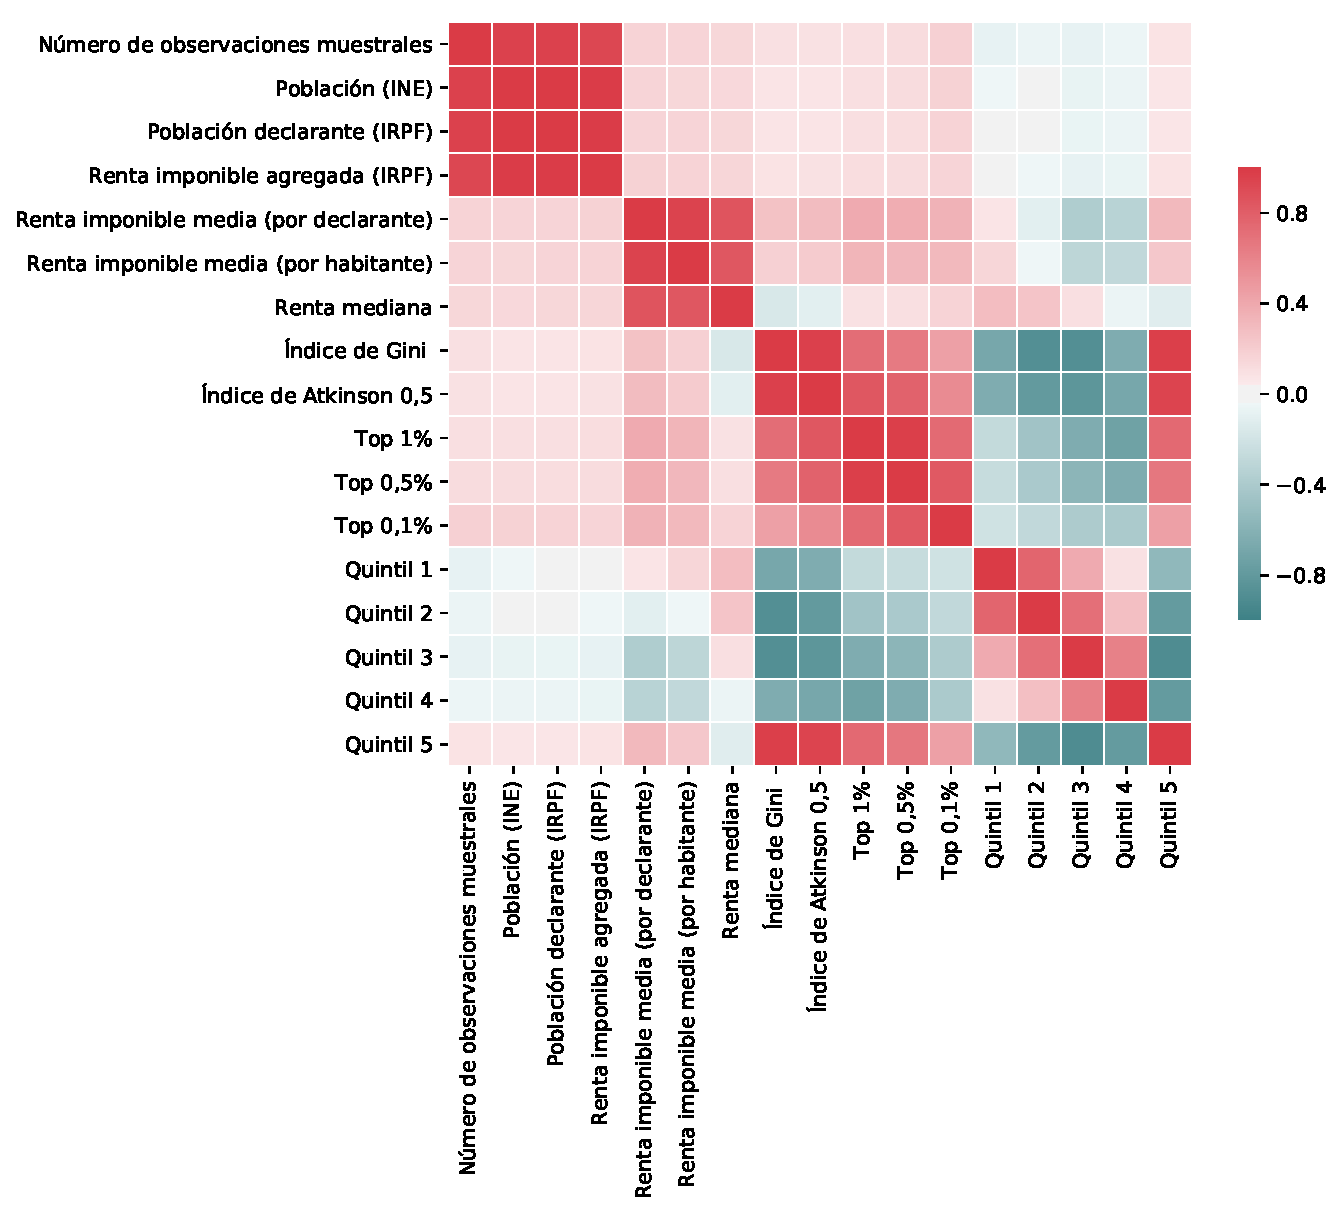
\includegraphics[width=\columnwidth]{Correlaciones1}
	\caption{Correlaciones entre todos los campos numéricos.}
	\label{fig:correlaciones1}
\end{figure}

\begin{itemize}
	\item El número de observaciones muestrales, si bien puede ser relevante desde el punto de vista de la recogida de los datos, no lo es tanto en este caso, por lo que se prescindirá de este campo.
	\item Los índices de Gini y de Atkinson son indicadores de desigualdad y ambos están muy correlacionados entre sí, por lo cual se puede optar por eliminar uno de los dos. De manera arbitraria se ha escogido eliminar el índice de Gini.
	\item Los quintiles son útiles para saber cómo está distribuida la renta dentro del propio municipio, pero se necesitan todos los campos para sacar una idea general. Todos están bastante correlacionados (inversa o directamente) con el índice de Atkinson, lo que invita a pensar que la distribución de los mismos está totalmente relacionada con la desigualdad que hay en el municipio, por lo que son campos de los que se pueden prescindir. En el caso de los top, la información que aportan es similar, por lo que también han sido descartados.
	\item Se ha considerado que conocer el número de declarantes puede ser interesante en este problema, sin embargo la cantidad total de los mismos no lo es tanto, por lo que se ha creado un campo nuevo: el porcentaje de población declarante, el cual se ha obtenido la población declarante entre la población total.
	\item La renta agregada no es muy relevante, ya que depende mucho de la población del municipio. En su lugar es mejor seleccionar o bien la renta media por declarante o la renta media por habitante. De manera arbitraria se ha elegido la renta media por declarante. La renta mediana se ha descartado por tener mucha correlación con la renta media.
\end{itemize}

Tras hacer esta selección, los campos que han quedado son ``Población INE '', ``Renta imponible media por declarante '', ``Índice de Atkinson 0.5'' y ``Porcentaje de Poblacion Declarante''. Estos campos prácticamente no están correlacionados entre sí tal y como se puede ver en la figura \ref{fig:correlaciones2}, lo cual los hace bastante útiles para el clustering.

\begin{figure}
	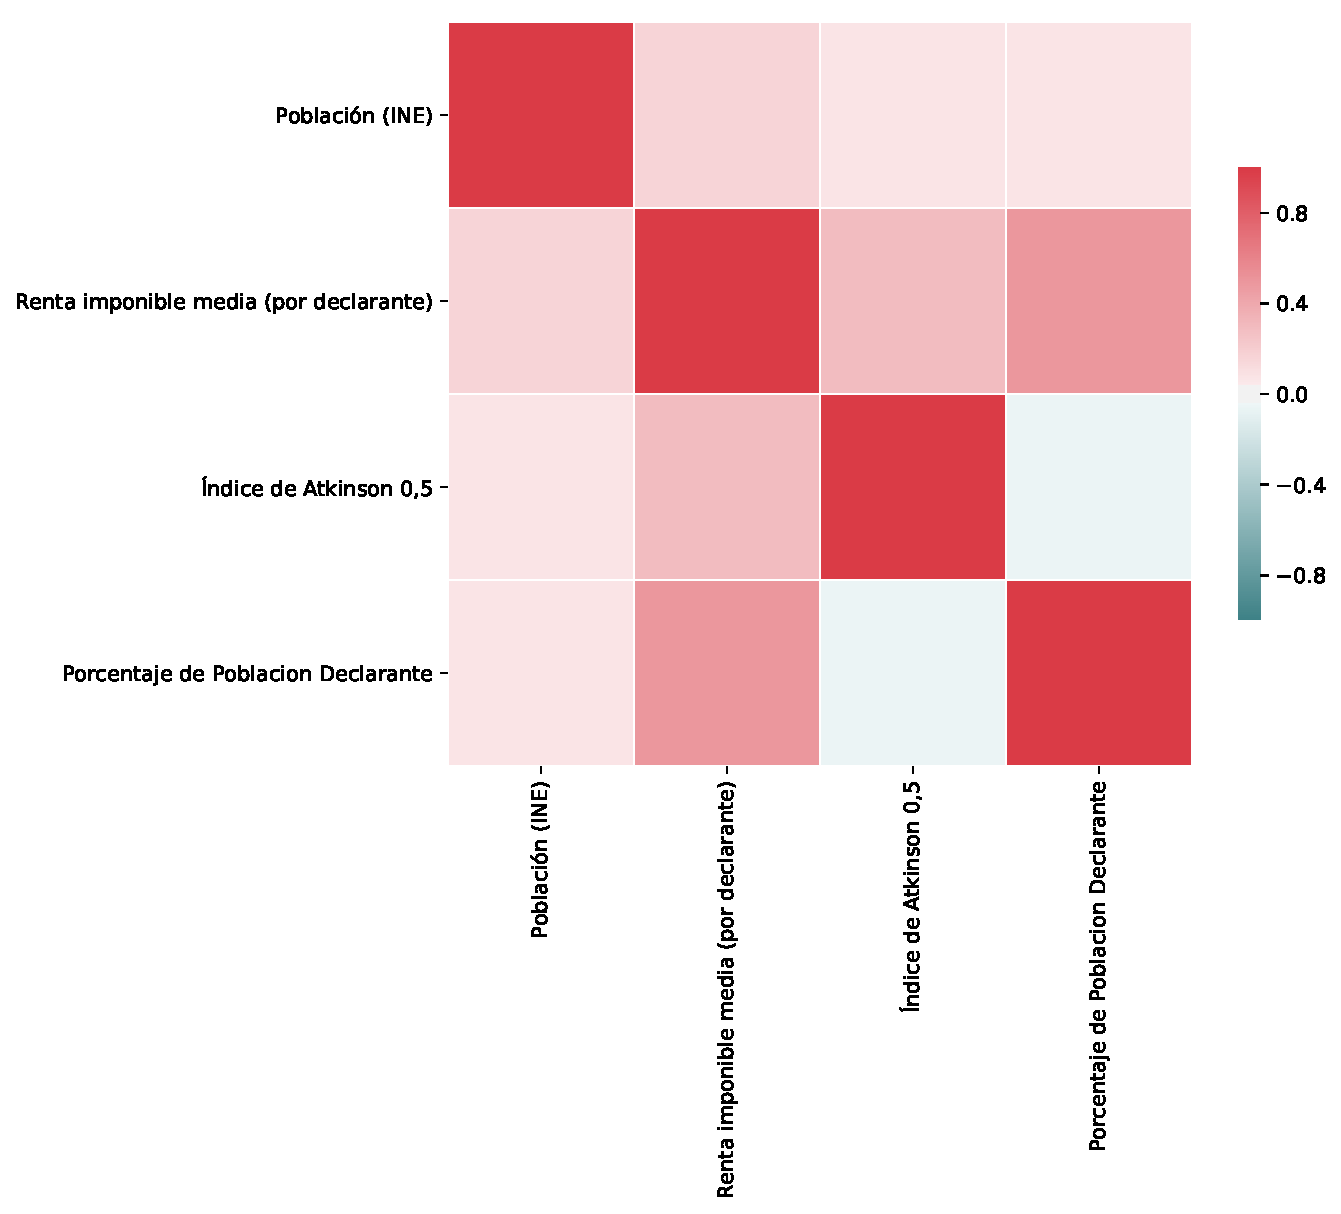
\includegraphics[width=\columnwidth]{Correlaciones2}
	\caption{Correlaciones entre los campos seleccionados para usarse en el clustering.}
	\label{fig:correlaciones2}
\end{figure}

\subsection{PCA}
Con el fin de poder mostrar gráficamente la disposición de los datos, se ha aplicado un Análisis de Componentes Principales a las columnas seleccionadas. El ratio de varianza explicado por el PCA vale 0.847, por lo que se considera que la representación será bastante fiel a la realidad. La figura \ref{fig:pca} muestra la representación gráfica del PCA. En ella se puede apreciar que los datos están especialmente concentrados en un punto desde el cual se van dispersando hacia casos más extremos.

\begin{figure}
	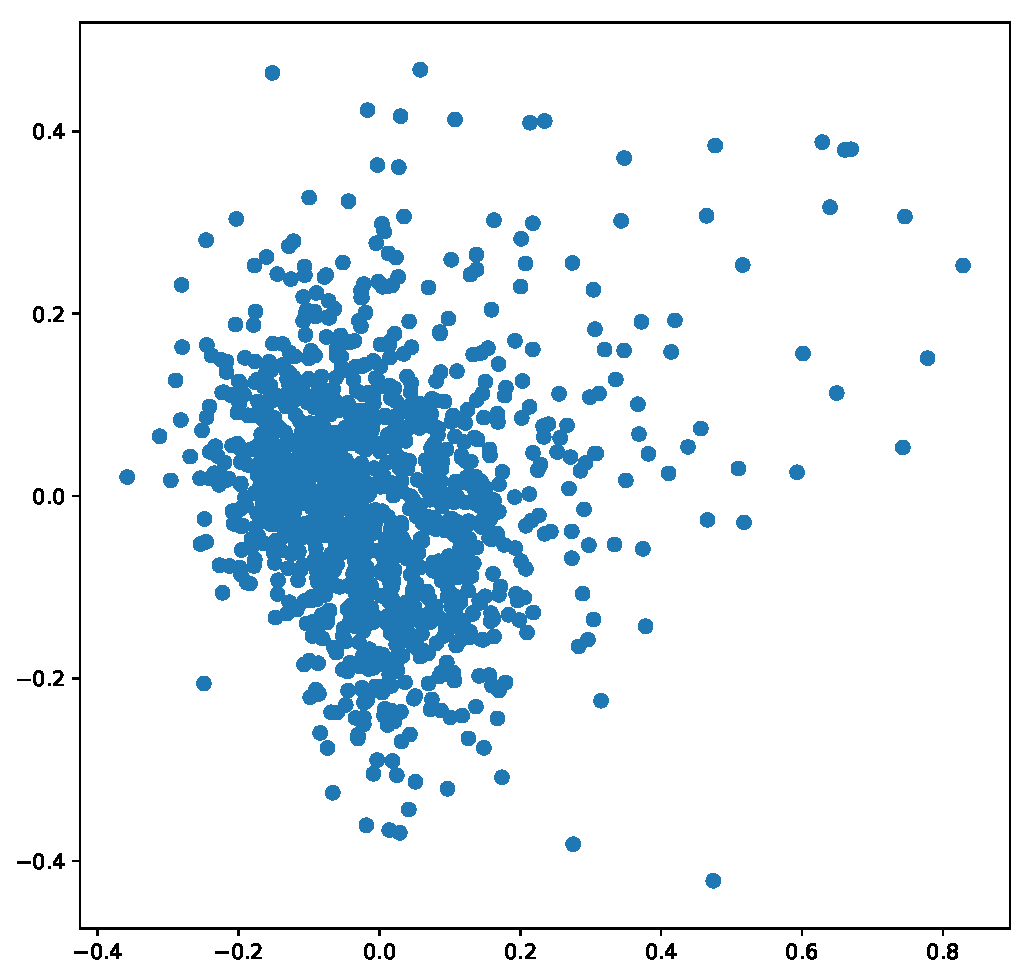
\includegraphics[width=\columnwidth]{pca}
	\caption{Gráfico mostrando la representación gráfica en 2D de las columnas seleccionadas.}
	\label{fig:pca}
\end{figure}

\section{Clustering}
En esta etapa se ha aplicado el algoritmo para agrupar los datos en diferentes clusters. En esta segunda fase se ha utilizado el lenguaje de programación R y el paquete 'kohonen'. El clustering se puede ejecutar mediante el script ``clustering.R''.

Antes de meter los datos al algoritmo se les ha aplicado una normalización min-max. Además se ha usado un logaritmo en base 10 al campo de la población. Esto se hace debido a que hay mucha diferencia entre las ciudades que más población tienen y las demás, lo cual hace que a la hora de agruparlas el clustering pueda considerar que una ciudad de 50.000 habitantes está cerca de una de 6.000 porque en comparación con Madrid, que tiene 6 millones, ambas tienen casi lo mismo.

\begin{figure}
	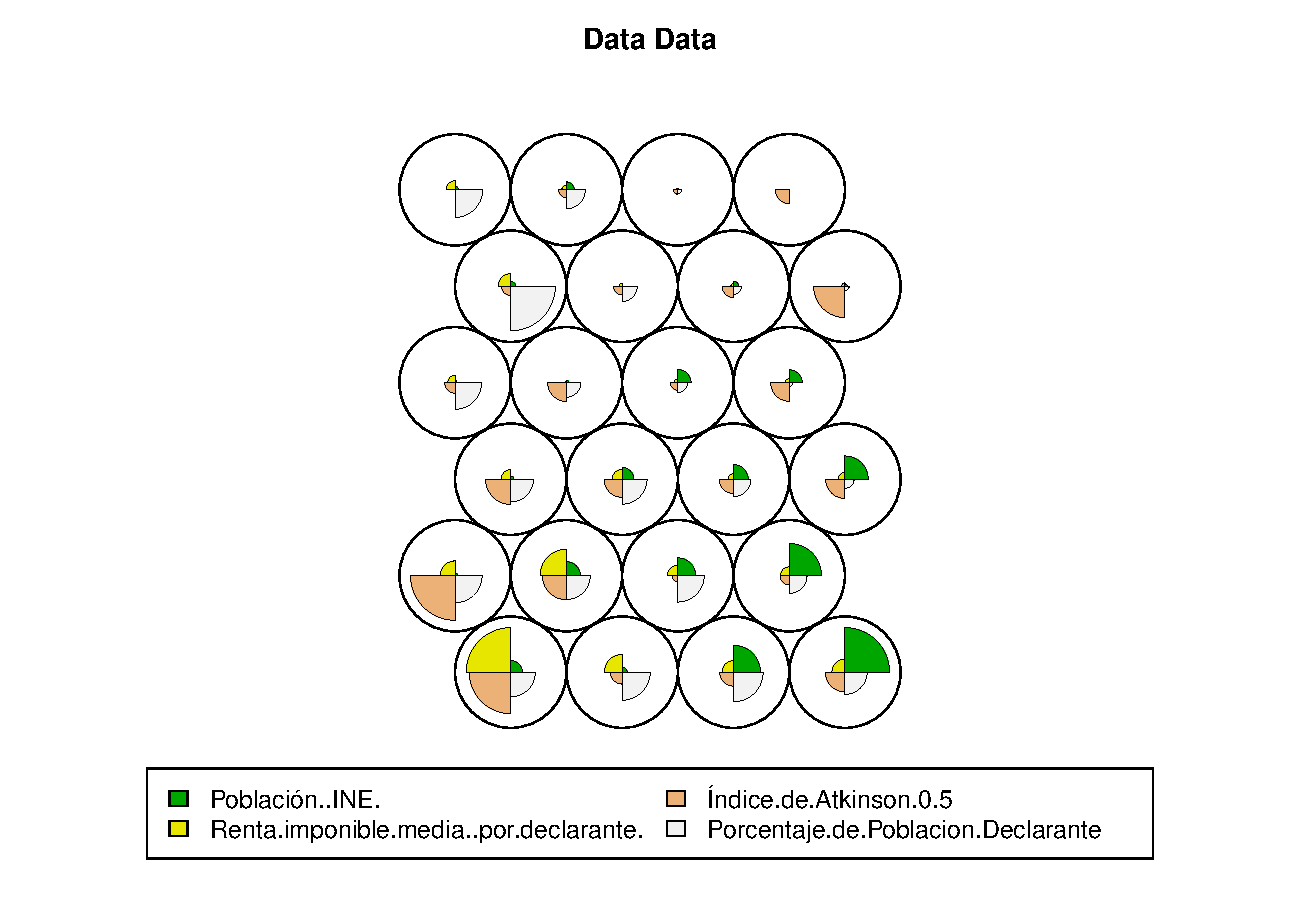
\includegraphics[width=\columnwidth]{mapaKohonen}
	\caption{Mapa de autoorganizado ya entrenado.}
	\label{fig:kohonen}
\end{figure}

Para la parametrización del mapa autoorganizado se ha decidido utilizar una red de 6x4 neuronas, con topología hexagonal y no toroidal. Para elegir esta parametrización se han probado varias hasta obtener una con unos resultados interesantes. Aún así, para validar la red neuronal se ha comprobado que la calidad, el número de elementos y la convergencia del aprendizaje fueran aceptables. En la figura \ref{fig:kohonen} se pueden ver los grupos que se han generado una vez entrenada la red.

El hecho de utilizar tantos grupos hace que haya algunos bastante similares, sin embargo, también permite poder detectar más fácilmente aquellos grupos que difieren notablemente del resto. Además, al tratarse de un mapa autoorganizado, es normal que se utilicen más grupos de los que se usarían con otras técnicas.

\subsection{Análisis de grupos}

Tras haber analizado distintos grupos que ha generado el clustering, se han encontrado algunos patrones interesantes:
\begin{itemize}
	\item \textbf{Grupo con más población(el 4)}: Este grupo se trata del que contiene las ciudades más grandes de España. Es relevante que prácticamente todas las ciudades grandes tienen la misma desigualdad, renta y porcentaje de declarantes a excepción de Barcelona y Madrid, en las cuales difieren un poco más.
	\item \textbf{Grupo con mayor renta media y mucha desigualdad(el 1)}: Estos son los pueblos más ricos de España, que coincide con y además son los segundos que mayor desigualdad presentan. Resulta llamativo el hecho de que todos estén alrededor de Madrid o Barcelona.
	\begin{figure}
		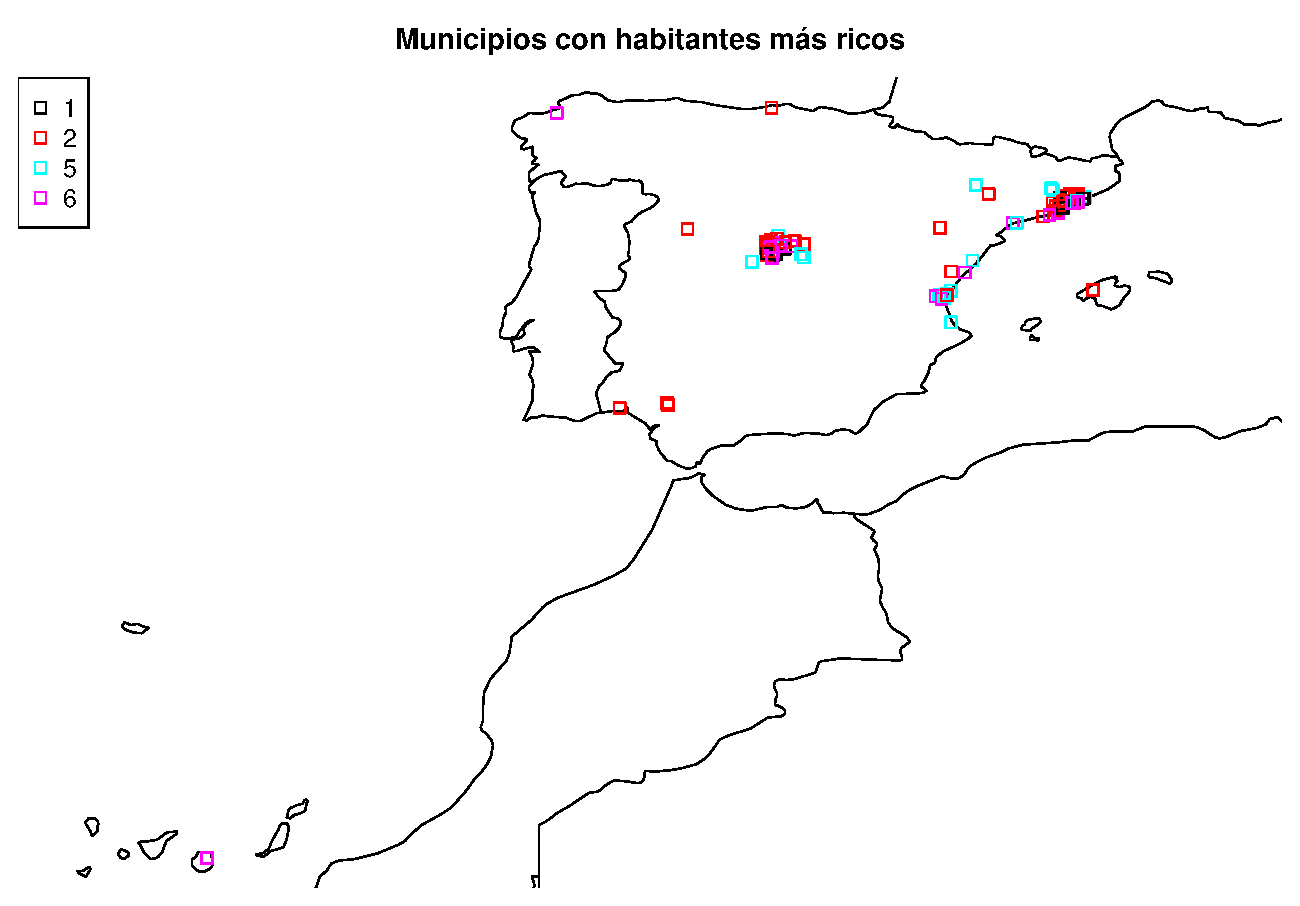
\includegraphics[width=\columnwidth]{mapaRicos}
		\caption{Mapa de España que muestra los municipios pertenecientes a los grupos con mayor renta media.}
		\label{fig:mapaRicos}
	\end{figure}
	\item \textbf{Grupos con mayor renta media (el 1, el 2, el 5 y el 6)}: Estos grupos, a parte de ser los que más renta media tienen, llaman la atención por coincidir en dos cosas más. La primera es que ninguno tiene demasiados habitantes y la segunda es que están todos situados en torno a la misma zona geográfica, tal y como se ve en la figura \ref{fig:mapaRicos}.
	\item \textbf{Grupo con mayor desigualdad y con poca población(el 5):} Los municipios pertenecientes a este grupo son, en su mayoría, pueblos que no son especialmente ricos, pero en los que hay algunas personas que amasan grandes fortunas.
	\item \textbf{Grupo con poca población, poca renta, poca desigualdad y alto porcentaje de población declarante(el 17)}: La mayoría de los municipios de este grupo se tratan de pueblos que estaban en proceso de crecimiento demográfico y que se encuentran cerca de núcleos urbanos(ciudades dormitorio).
	\begin{figure}
		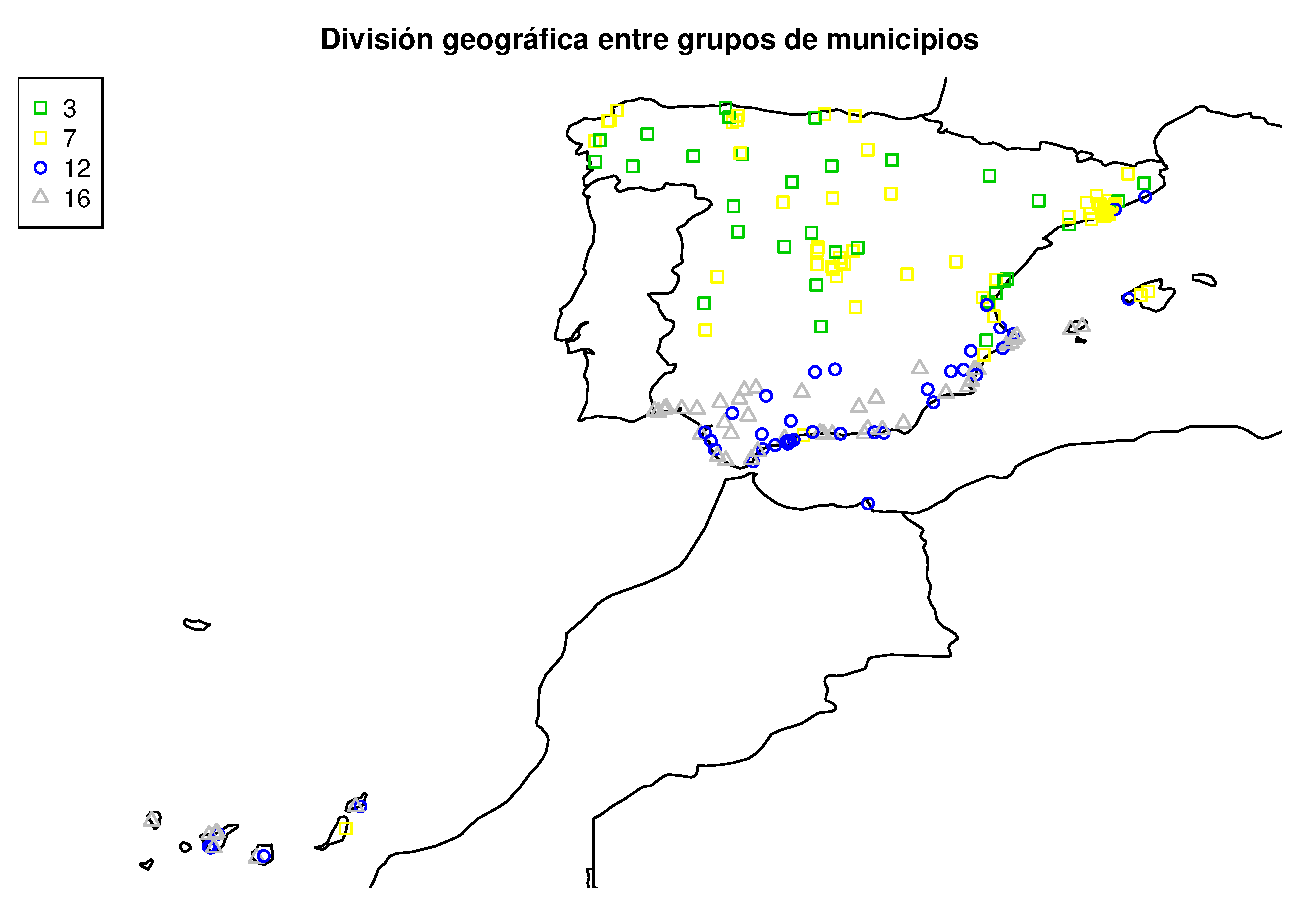
\includegraphics[width=\columnwidth]{dosEspanas}
		\caption{Mapa de España que muestra los municipios pertenecientes a diversos grupos que se encuentran en dos zonas bastante diferenciadas de España.}
		\label{fig:dosEspanas}
	\end{figure}
	\item \textbf{Los 2 grupos que tienen una cantidad intermedia de población y desigualdad(el 12 y el 16)}: Estos grupos tienen una peculiaridad bastante interesante y es que en ambos los municipios se encuentran sobre todo en Andalucía y Murcia tal y como se puede ver en la figura \ref{fig:dosEspanas}.
	\item \textbf{Los grupos que están en la columna 3 de las dos primeras filas desde abajo(el 3 y el 7)}: Estos grupos tienen una población y porcentaje de declarantes notables. Lo interesante de estos grupos, como se puede ver en la figura \ref{fig:dosEspanas}, es que ocupan una sección geográfica separada claramente de los grupos que se han visto en el punto anterior. En general estos pueblos tienen una renta media algo mayor que en los anteriores y menor desigualdad.	
	\begin{figure}
		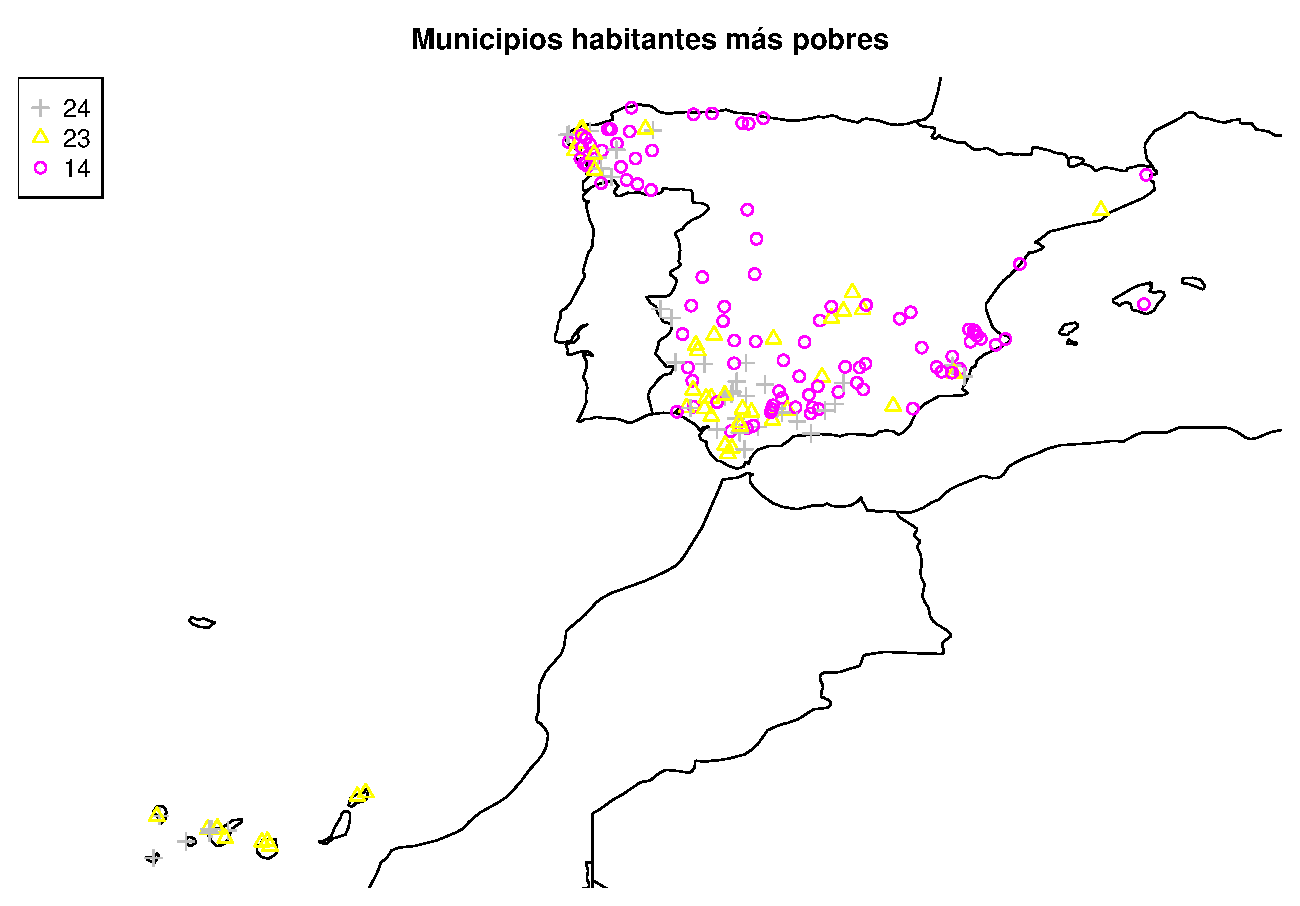
\includegraphics[width=\columnwidth]{mapaPobres}
		\caption{Mapa de España que muestra los municipios pertenecientes a los grupos con menor renta media.}
		\label{fig:mapaPobres}
	\end{figure}
	\item \textbf{Los 3 grupos con habitantes más pobres (el 14, el 23 y el 24)}: Tal y como muestra la figura \ref{fig:mapaPobres}, los pueblos más pobres se encuentran sobre todo en la mitad sur de la península, en Galicia y en Canarias, aunque también hay algunos en Extremadura y Castilla y León.
\end{itemize}

\end{document}
